\documentclass[12pt]{article}

\usepackage[utf8]{inputenc}
\usepackage{geometry}
\geometry{a4paper,scale=0.75}
\linespread{1.5}
\usepackage{graphicx} 
\usepackage{float} 
\usepackage{subfig} 
\usepackage{enumerate}
\usepackage{enumitem}
\usepackage{amsmath}
\usepackage{array}
\usepackage{booktabs}
\usepackage{multirow}
\usepackage{amsfonts}
\usepackage[english]{babel}
\usepackage{amsthm}
\usepackage{dcolumn}
\usepackage{multicol}
\usepackage{stfloats}
\usepackage{lscape}
\usepackage[figuresright]{rotating}
\RequirePackage{pdflscape}
\usepackage[toc,page]{appendix}
\usepackage{geometry}
\usepackage{longtable}
\usepackage{comment}
\usepackage{xcolor}

% -------- enumerated sub-labels (a), (b), … --
\usepackage{enumitem}
\setlist[enumerate,1]{label=(\alph*),ref=\alph*}
% ---------------------------------------------

\usepackage{hyperref}
\hypersetup{hidelinks,
	colorlinks=true,
	allcolors=black,
	pdfstartview=Fit,
	breaklinks=true}
\usepackage{csquotes}
\usepackage{natbib}
\bibliographystyle{apalike}
\newtheorem{definition}{Definition}
\newtheorem{theorem}{Theorem}
\newtheorem{proposition}[theorem]{Proposition}
\newtheorem{lemma}[theorem]{Lemma}
\newtheorem{corollary}[theorem]{Corollary}
\newtheorem*{remark}{Remark}
\newtheorem{example}{Example}
\newtheorem{exercise}{Exercise}
\newtheorem{assumption}{Assumption}[section] % number within sections


\begin{document}

\begin{center}
    ECON 3123: Macroeconomic Theory I\\
    {\large \textbf{Tutorial Note 4: Basic IS-LM Framework}}\\
    Teaching Assistant: Harlly Zhou
\end{center}

\subsection*{Derivation of IS-LM Model}
Recall that in the goods market, the deamnd for goods is
\[ Z = C + I + G. \]
Recall that consumption depends on disposable income $Y-T$. And in reality, investment depends on output and interest rate:
\[ I = I (Y,i),\]
where $I$ increases with $Y$ and decreases with $i$. (Think about the intuition.)

Then we rewrite the demand as
\[ Z = C(Y-T) + I(Y,i) + G.\]
At equilibrium, we have
\[ Y = Z.\]
This determines the equilibrium output $Y^*$. When the nominal interest rate increases, the investment will decrease, shifting the $ZZ$ curve downwards. We have the new equilibrium output $Y'$, shown as Figure \ref{fig:is_01}.

\begin{figure}[htp]
    \centering
    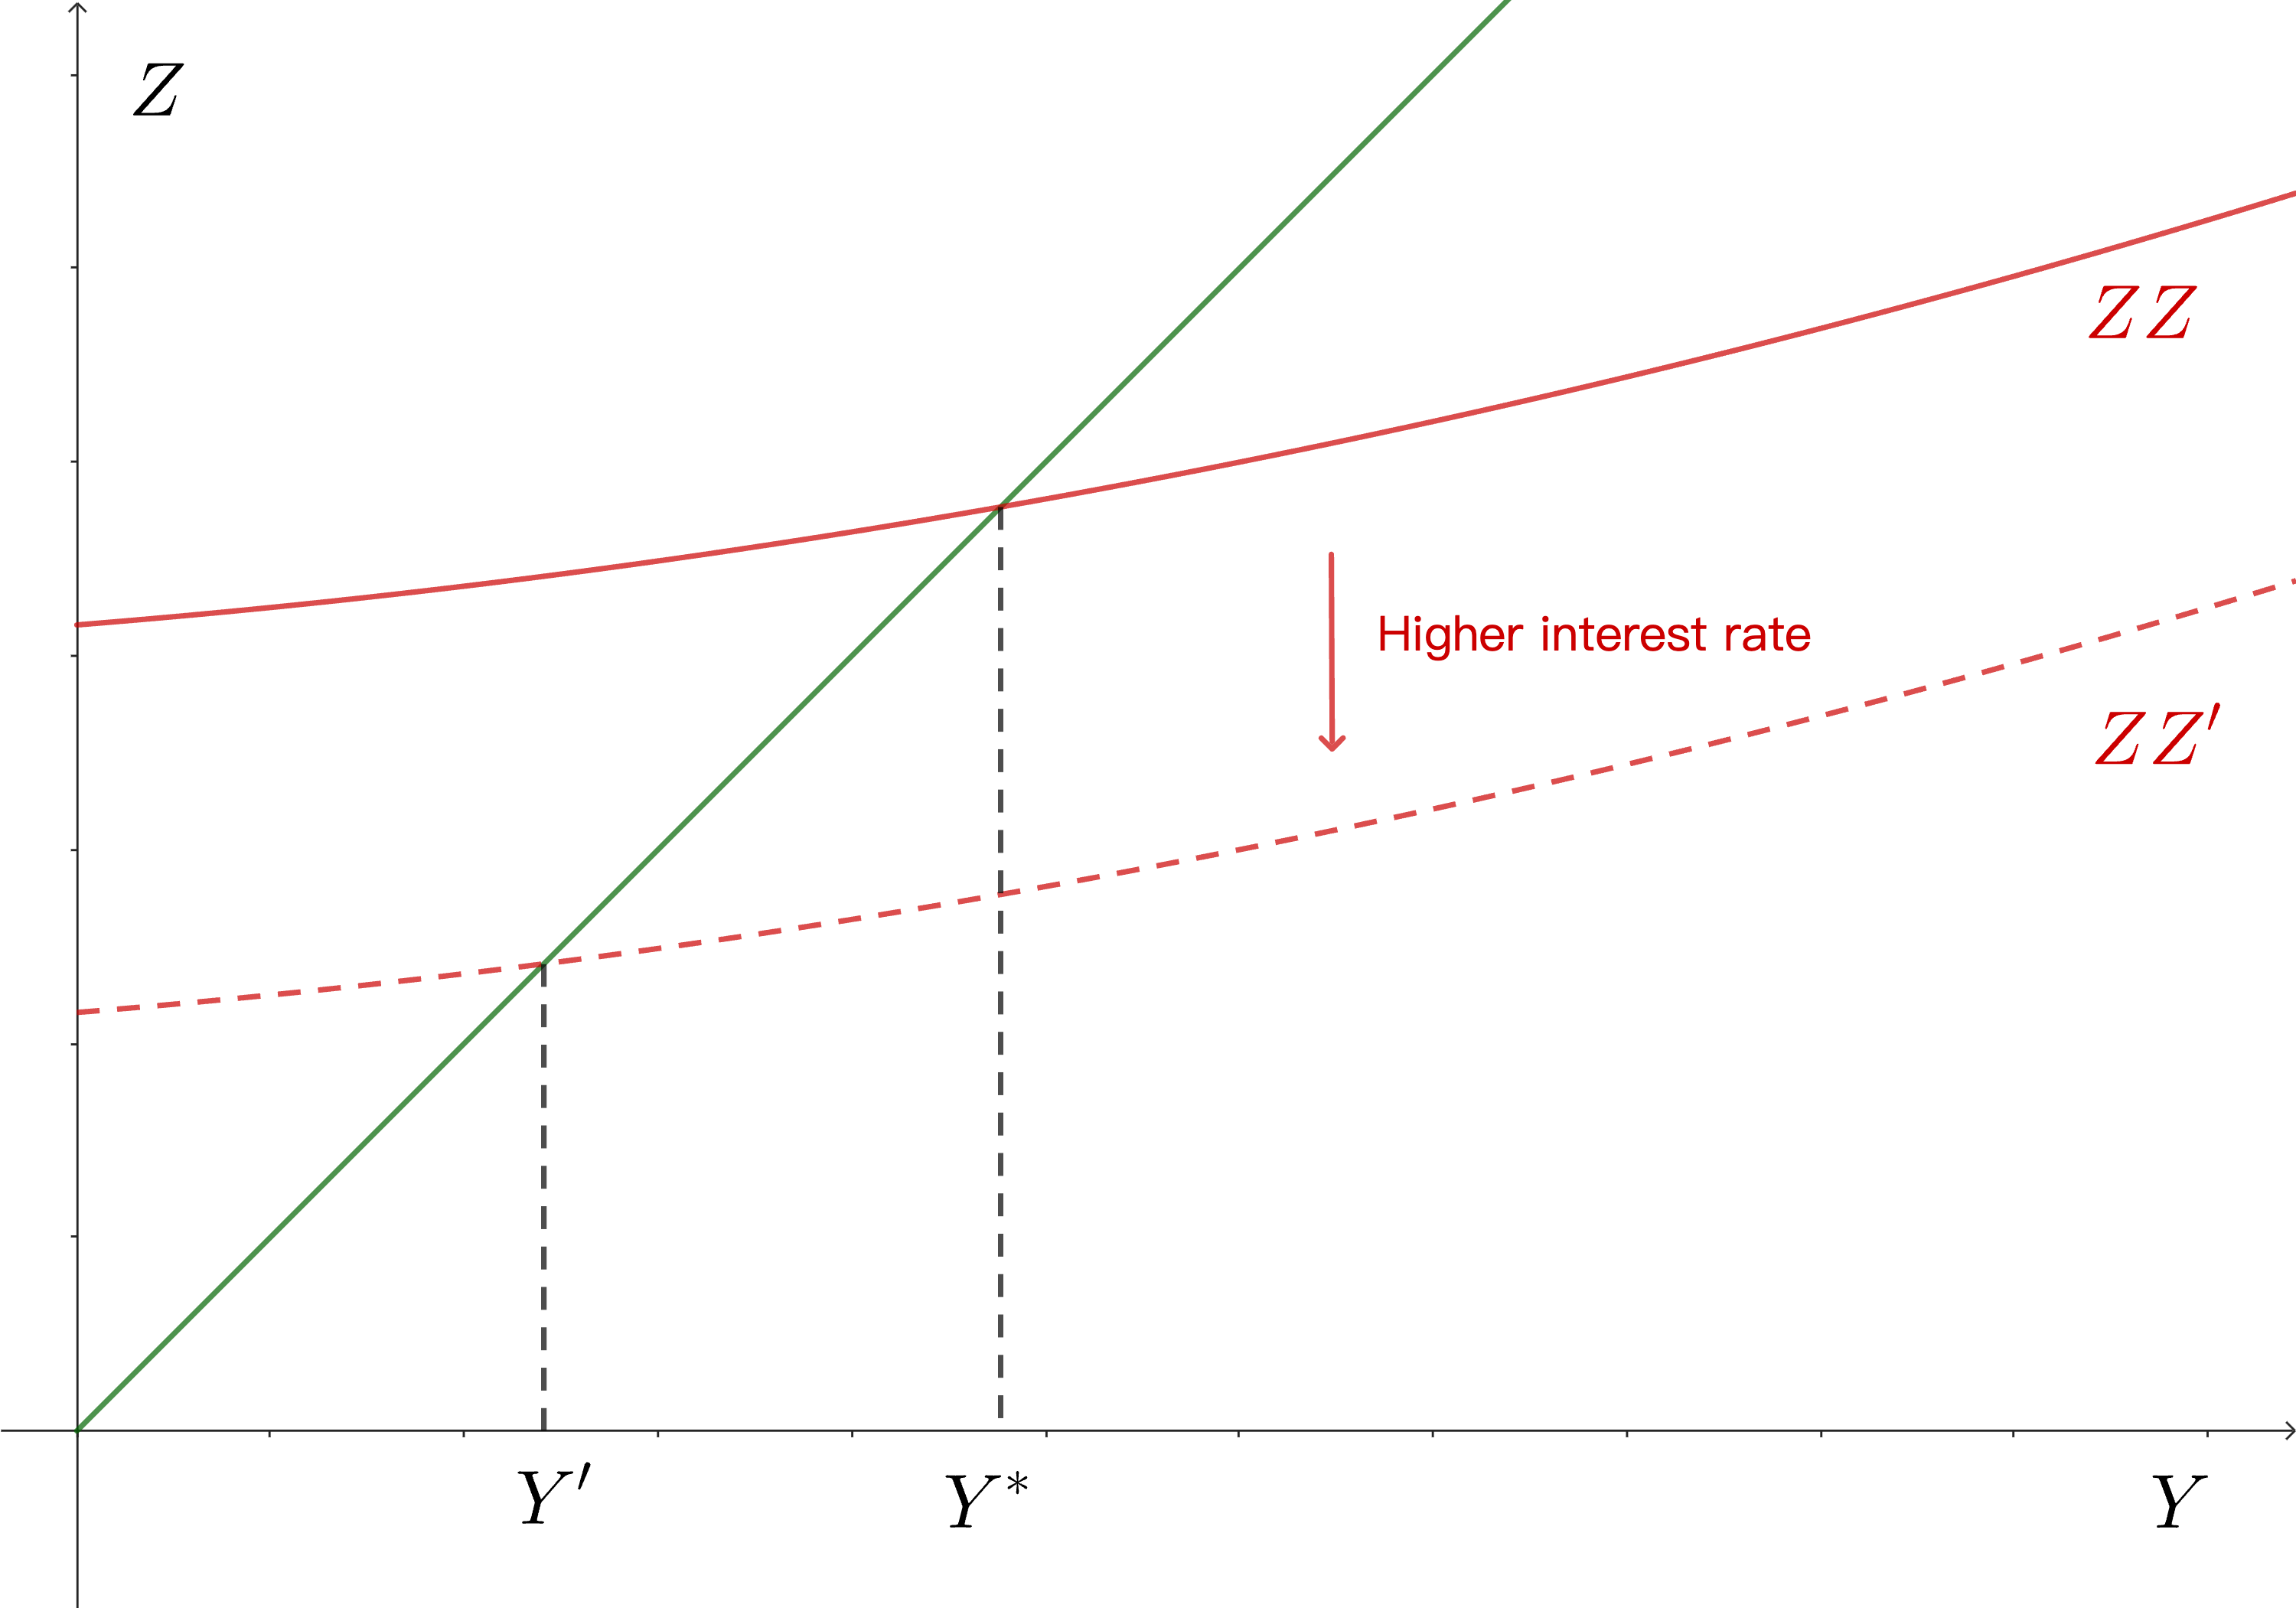
\includegraphics[width=0.6\textwidth]{is_01.png}
    \caption{Goods Market Equilibrium}
    \label{fig:is_01}
\end{figure}

If we put the interest rate and the output together, then we get the IS relation (Figrue \ref{fig:is_02}).\

\begin{figure}[htp]
    \centering
    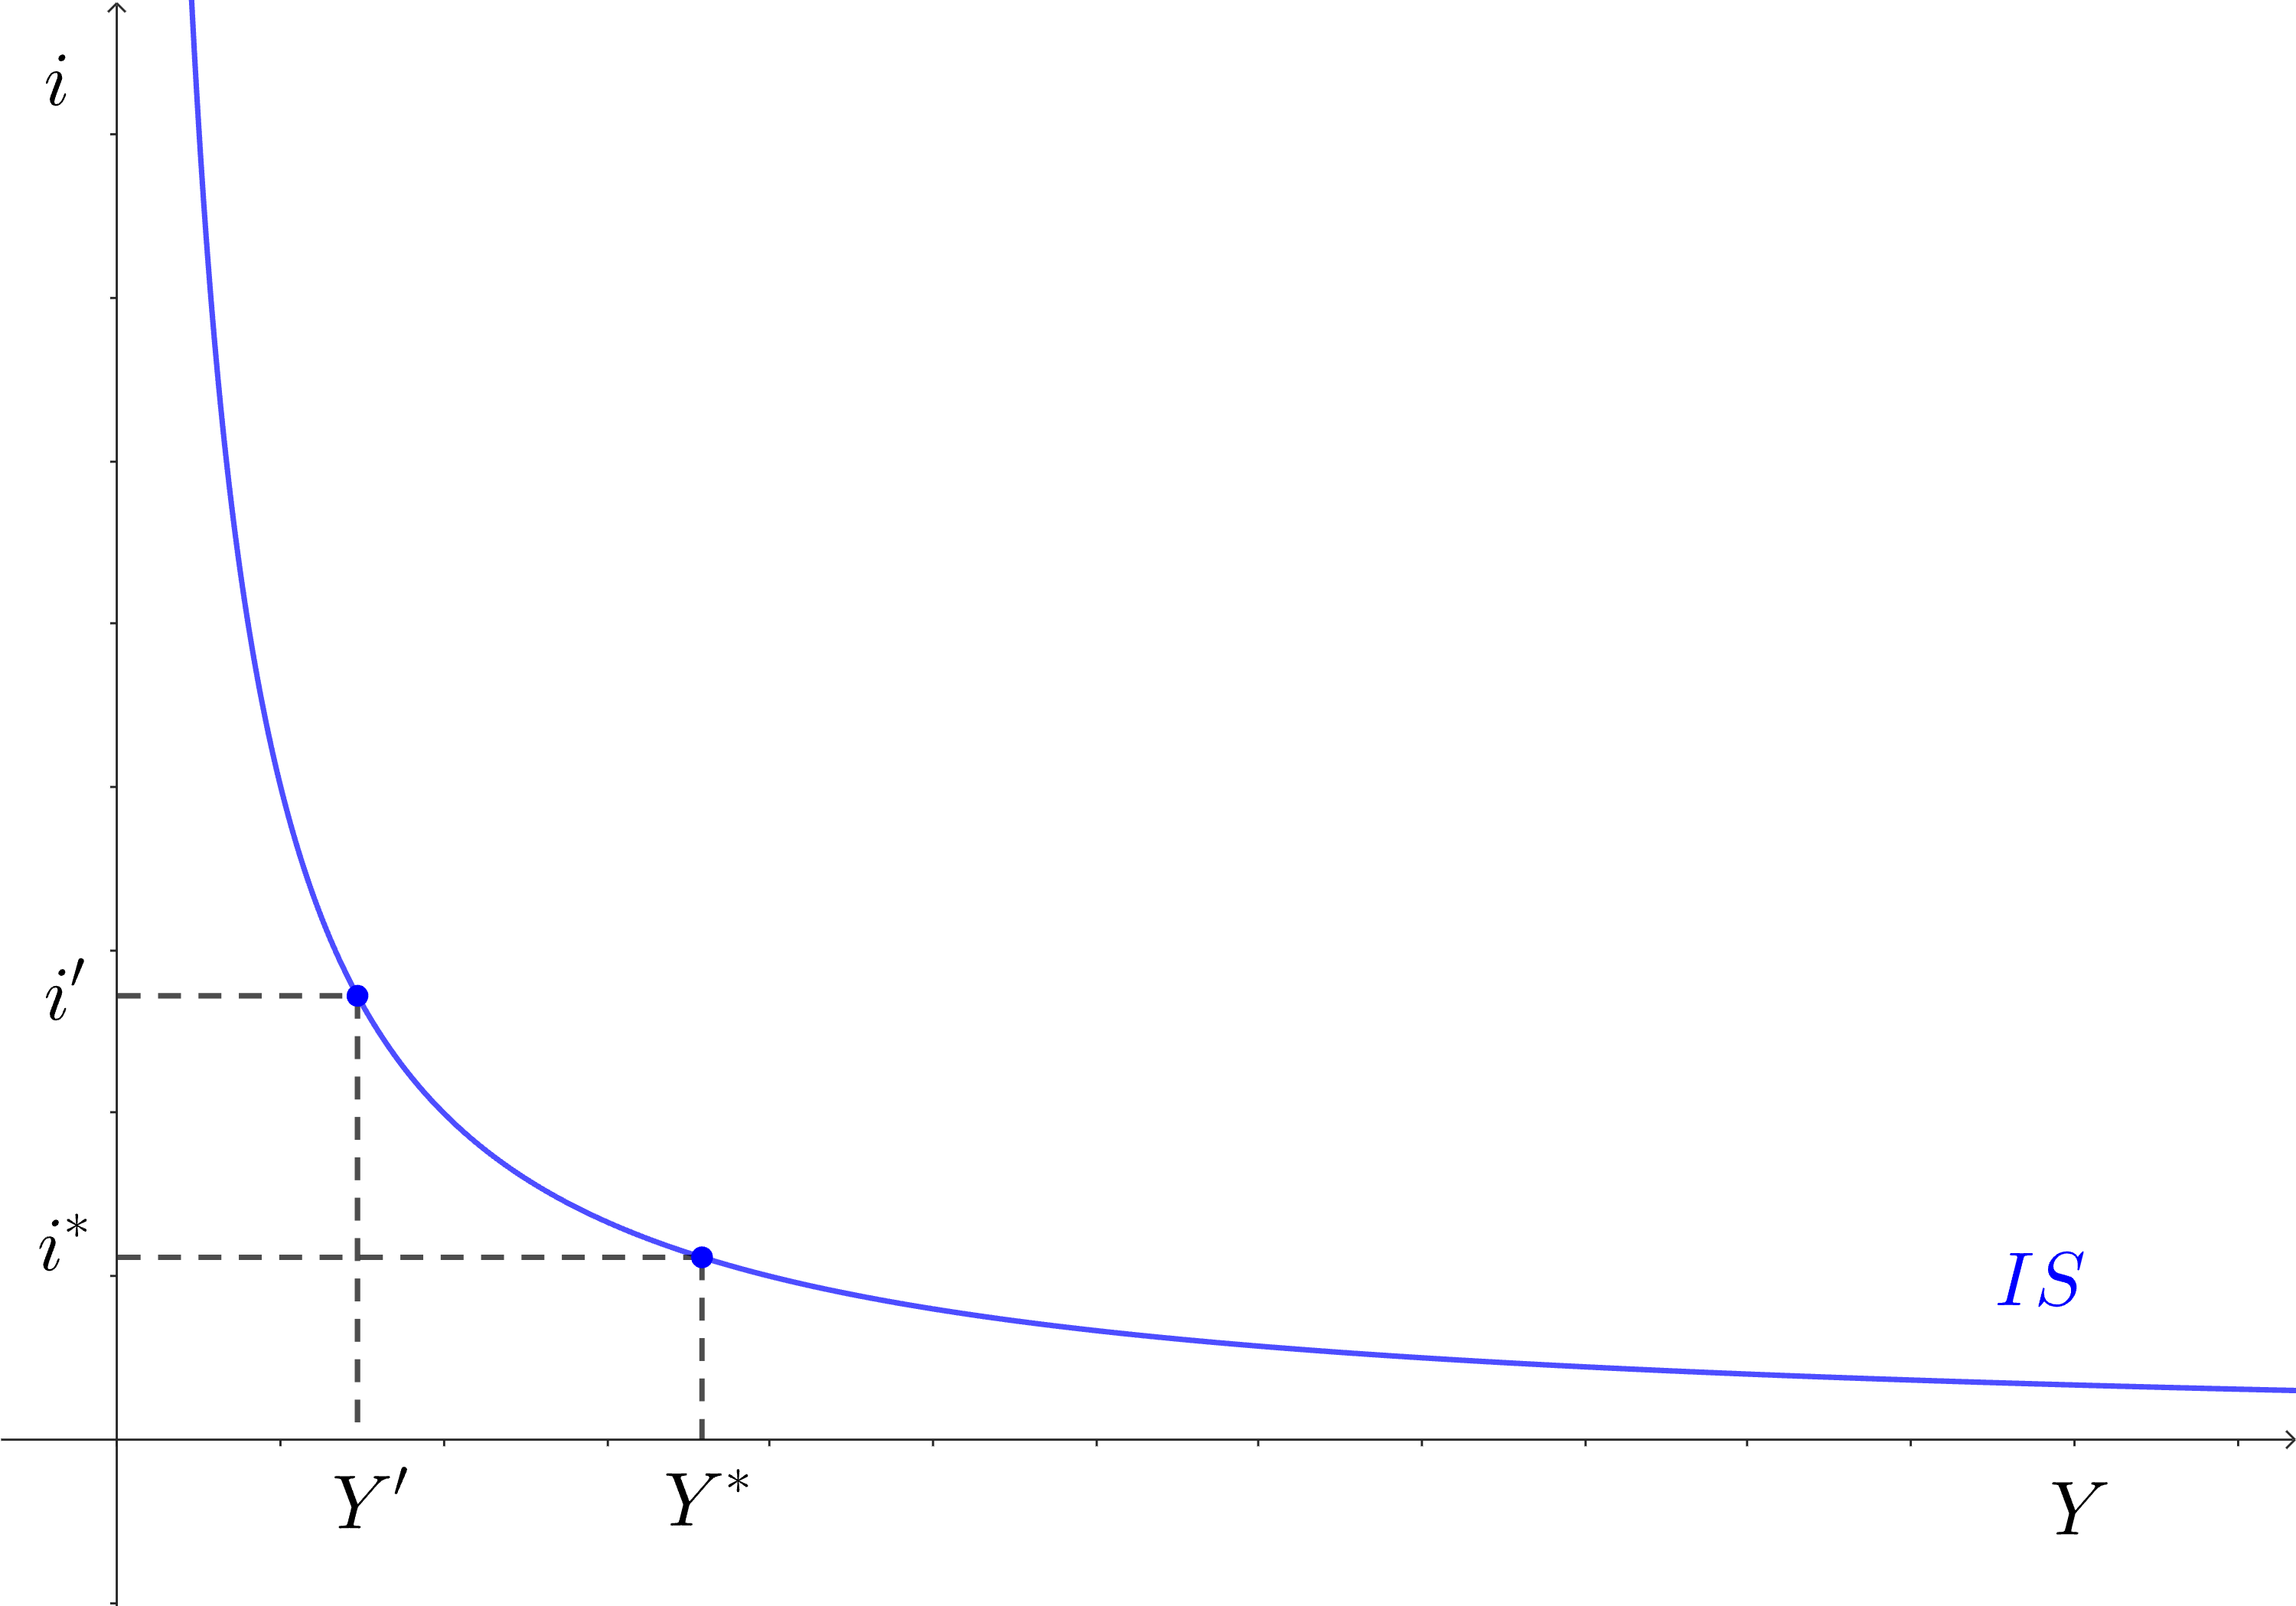
\includegraphics[width=0.6\textwidth]{is_02.png}
    \caption{Deriving IS curve from goods market equilibrium}
    \label{fig:is_02}
\end{figure}

Note that all the pairs $(i, Y)$ is a pair of \textbf{equilibrium} values of nominal interest and output.

In the derivation of the IS relation, note that the output is measured in \textit{real temr}. Therefore, we should also use real term in the money market equilibrium to derive the \textbf{LM relation}. Recall that the nominal money demand is
\[M^d = \$ Y L(i)\]
for some decreasing function $L(i)$. The real money demand is
\[\frac{M^d}{P} = Y L(i).\]
At equilibrium, $M^d = M^S = M$. In the short run, we assume that prices are sticky. Hence, we have
\[ \frac{M}{P} = Y L(i).\]
Central banks adjust money supply $M$ to target an interest rate $i = \bar{i}$. Hence, the LM curve is a horizontal line. Putting together with the IS curve, we get Figure \ref{fig:is-lm}.

\begin{figure}[htp]
    \centering
    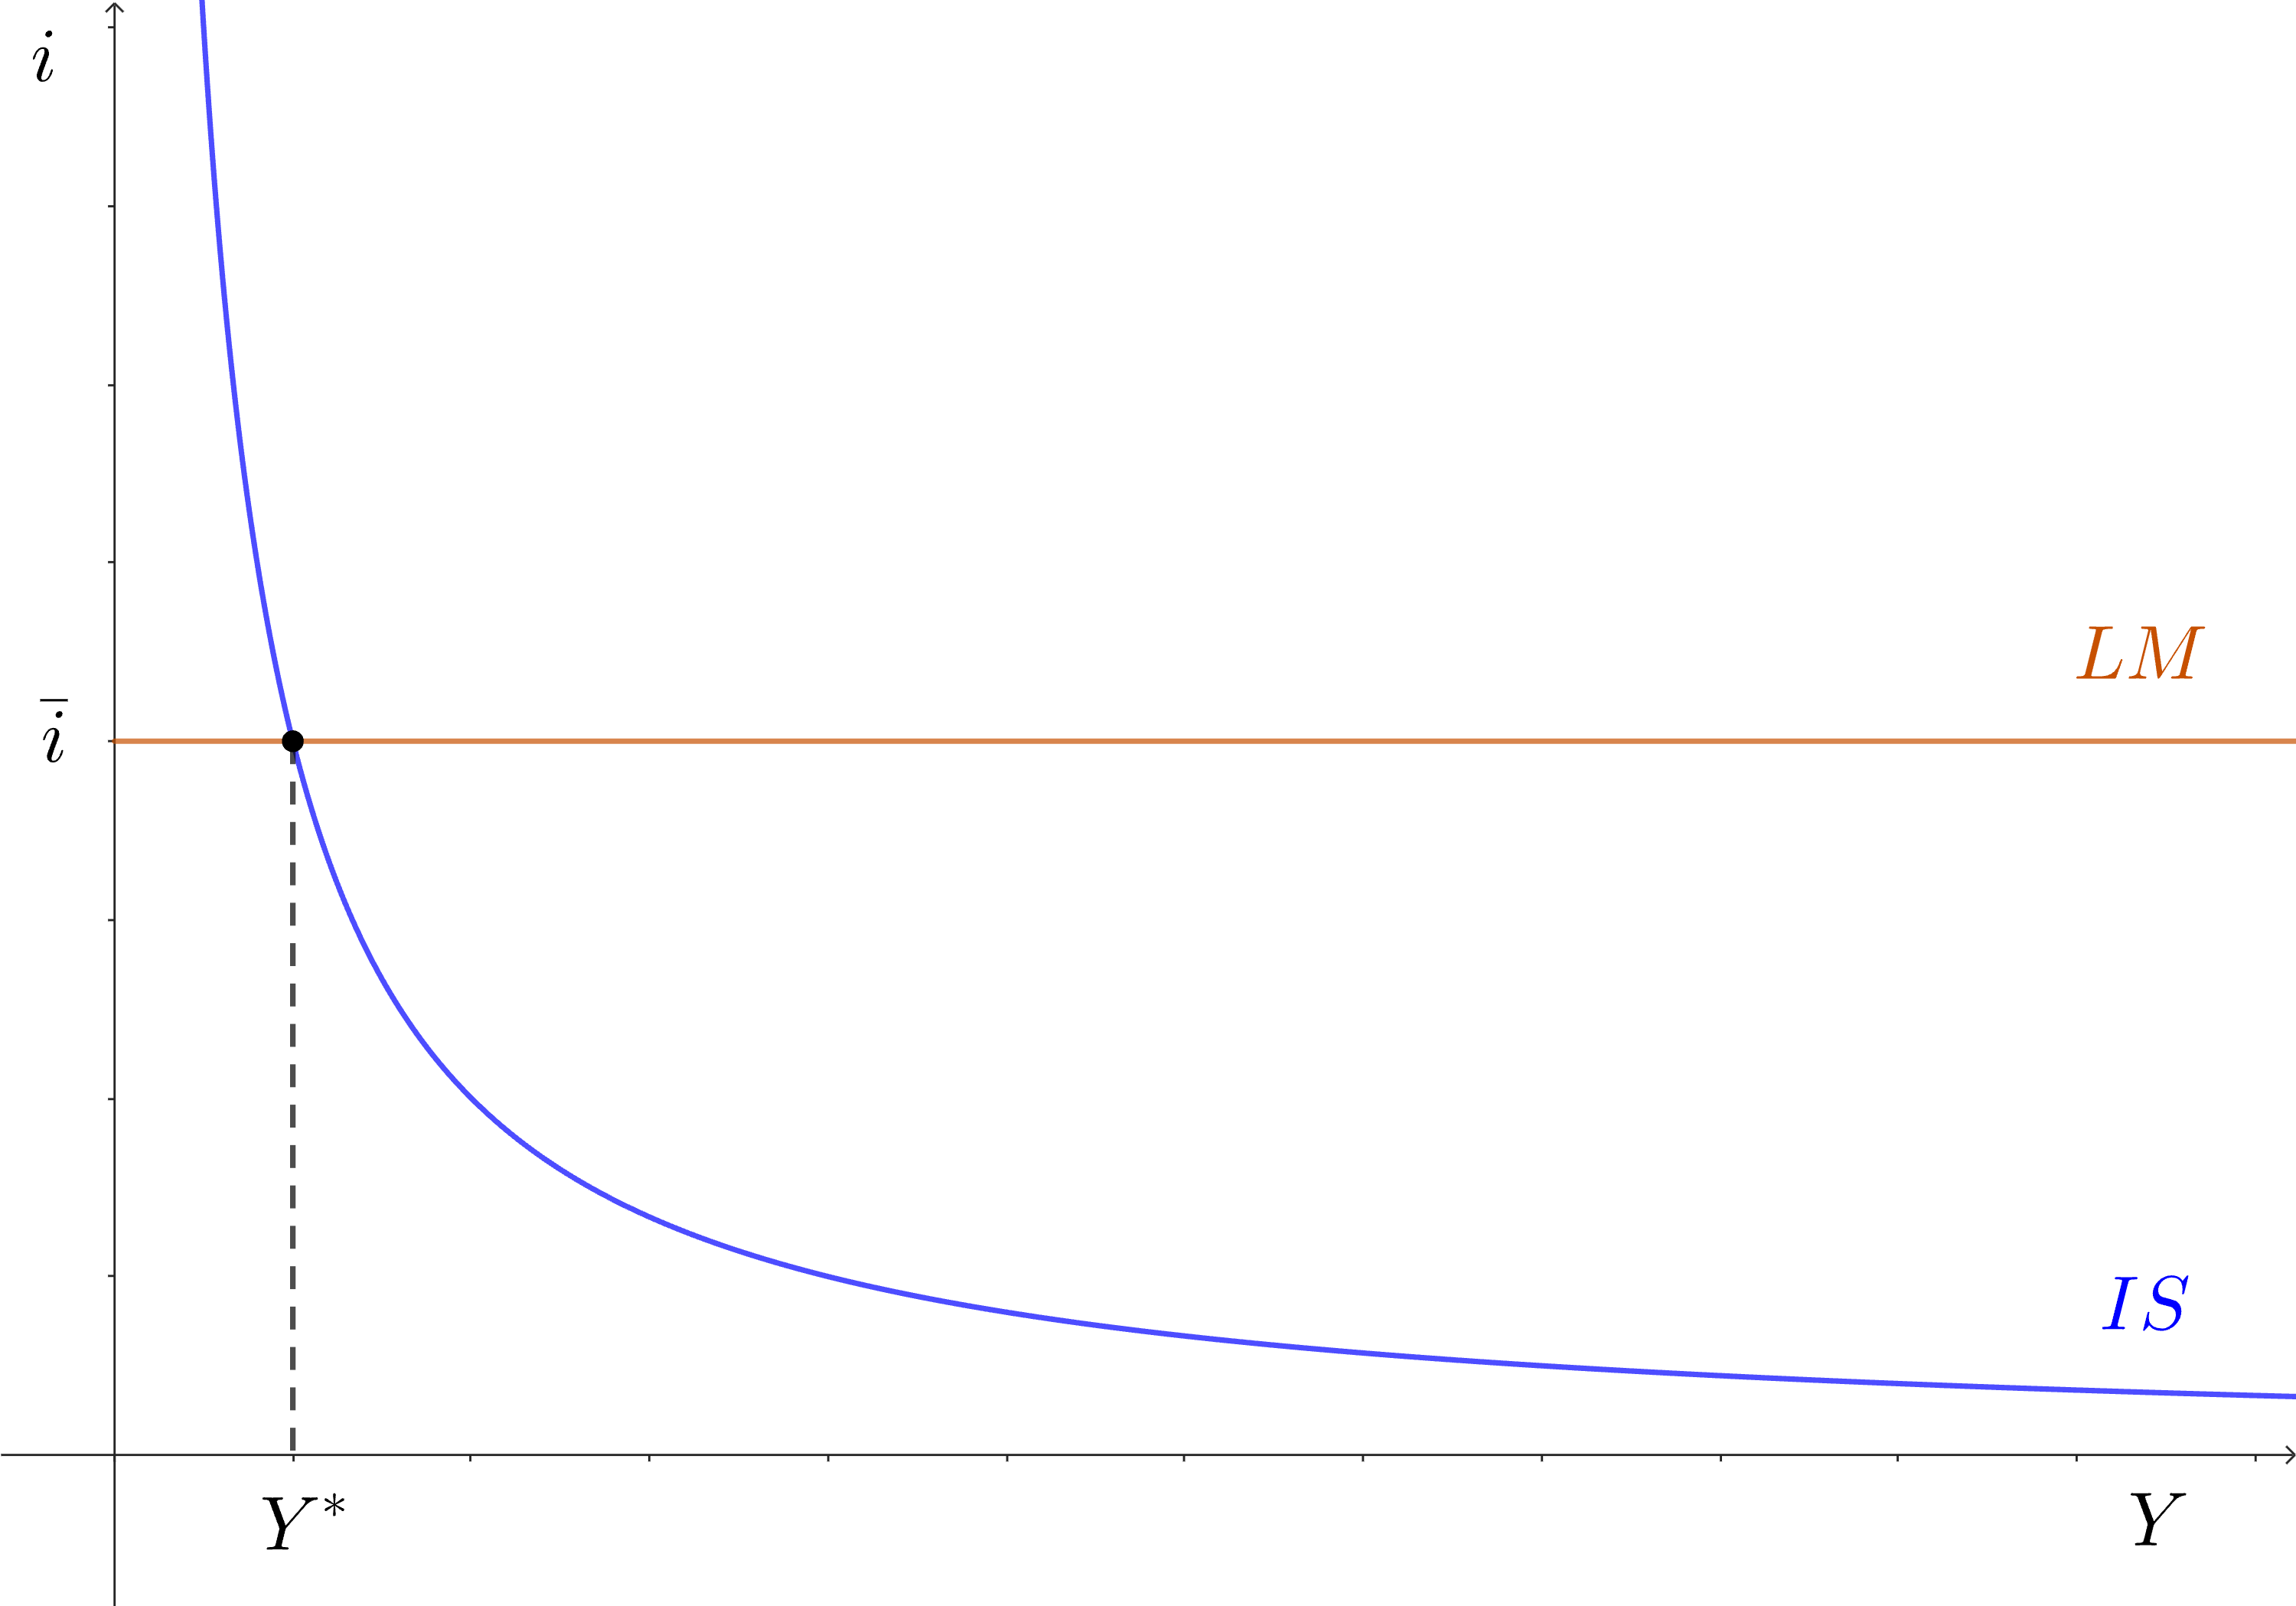
\includegraphics[width=0.6\textwidth]{is-lm.png}
    \caption{IS-LM Framework}
    \label{fig:is-lm}
\end{figure}

\begin{example}
    Suppose that the consumption behavior of people follows the following behavioral equation:
    \begin{align*}
        C = 0.8 (Y-T)
    \end{align*}
    and the investment follows the following:
    \begin{align*}
        I= 510 - 200 i.
    \end{align*}
    Suppose that government spending is 300, total export is 200, total import is 400, and the price level is 10.

    Suppose that the nominal money demand is
    \begin{align*}
        M^d = \$ Y (0.25 - i),
    \end{align*}
    and the government is targeting a nominal interest rate of $5\%$.

    Derive the IS relation and the LM relation. Use the IS-LM framework to derive the equilibirum output.
\end{example}


\end{document}